\iffalse
\begin{figure}[h]
	\centering
	\includegraphics[width=\columnwidth]{figures/teaser.pdf}
	% \caption{\textbf{\ours\ makes a pretrained VLA motion-aware.}
	% We study four dynamic bimanual tasks in which the target object is in motion
	% (\emph{far left}): Drop Catch, Bottle Handover, Flick Catch, and Wine Pour.
	% Conditioned on a single observation (\emph{red}), a standard VLA cannot
	% perceive how fast or in which direction objects are moving (red arrows,
	% ``?\,m/s''), so it cannot act reliably when the target is in motion.
	% \ours\ instead conditions the policy on two signals derived from recent
	% history, a compact summary of object motion and the policy's own recent
	% actions, letting it reason about how the scene is moving and complete the
 % to	task (\emph{green}).}
	\label{fig:teaser}
\end{figure}
\section{Introduction}
\label{sec:introduction}

A robot equipped with a capable VLA receives a bottle from a walking colleague. The person walks with the bottle at various speeds, and the robot must intercept it at the right moment. The policy is conditioned on a single snapshot: a frame captured when inference began, tens to even hundreds of milliseconds before any action executes. By the time the robot moves, the environment evolves: the object of interest might have moved, and the robot arm is elsewhere. The policy reaches for where the objects were based on the past position of the robot arm, not where it is going. The robot misses.

This is not just a latency failure, it is representational. Even with the newest possible frame, a single image encodes structure, not motion: the policy sees the bottle but not its velocity, so it knows it must grasp the bottle, yet cannot tell when. The ambiguity is in the input itself, not the timing.
  
A second form of ambiguity arises from the state itself. Two visually similar frames, one with a hand approaching at the start of the task, the other with it receding at the end, can be nearly perceptually identical, yet demand opposite actions. A policy conditioned on the current snapshot alone cannot distinguish them; conditioned on this ambiguous state, it produces an action that hedges over both cases, and the result is hesitation, mistiming, or failure. \textit{State aliasing, not reaction speed, is the primary obstacle to deploying VLAs in dynamic settings.}

Both kinds of ambiguity, motion and state, are symptoms of a single assumption: that the current snapshot is sufficient for action. This Markovian assumption underlies virtually every VLA today~\cite{pi0, pi05, openvla}. For quasi-static tasks where objects remain fixed during inference, it is a reasonable approximation. It fails structurally when motion enters the scene, whether from a moving object, a robot arm mid-swing, or a perturbation in progress. As the community develops stronger VLA foundations, the natural next question is whether they can operate in environments that do not hold still; the Markovian assumption imposes a ceiling that stacking more frames cannot break through.

The most obvious ``fix'', feeding more image frames as context, worsens the core problem. Additional frames lengthen the input, increasing inference time and widening the gap between what the policy observed and what is true at execution. Raw frames are also largely redundant: a reliable motion signal emerges only with enough history that inference cost becomes prohibitive. As most pretrained VLA backbones do not accept variable-length history, this route requires retraining from scratch, forfeiting the investment in existing models. We present a Temporal Encoding for Motion-aware Policy (\ours), which addresses these issues via two targeted additions to any pretrained VLA backbone, without modifying it: a compact summary of how the scene has moved, and a compact history of actions the robot has taken.

The first addition is a \textit{motion encoder}: a lightweight module that compresses a short observation window into a compact representation of scene flow, appended to the standard input without drastically increasing context length. In the Bottle Handover task, this distinguishes an approaching hand from a receding one, resolving the aliasing that causes the single-frame baseline to fail. The second is a \textit{compact joint history}: a short summary of the policy's own recent joint positions. \llm{The motion encoder captures how the scene is moving, addressing the motion ambiguity of fast, shifting targets; the joint history captures what the robot has recently done, addressing the state aliasing between perceptually similar phases of a task.} Both modules are task-agnostic and attach to any pretrained backbone without retraining.
%: the same configuration handles Flick Catch, Drop Catch, Bottle Handover, and Wine Pour.
We compare \ours\ against various baselines on a bimanual platform across four different dynamic tasks: Flick Catch (selecting and catching one of six human-flicked balls), Drop Catch (catching a ball the human swings horizontally), Bottle Handover (receiving a bottle from a walking person), and Wine Pour (following a human pour).

A complementary line of work addresses the execution side of the problem: asynchronous inference methods~\cite{rtc, vlash} decouple inference and execution, reducing the temporal gap between when a policy observes the world and when its actions take effect. These are orthogonal to \ours: asynchronous execution ensures predictions are applied at the right time, while \ours\ ensures the predictions themselves are motion-aware. In our experiments, \ours\ is built on top of an asynchronous backbone~\cite{vlash}, and the gain over the async-only baseline shows that motion-aware perception remains necessary even when timing is already addressed.


Our contributions are: (1) an efficient motion encoder and a compact joint history, two minimal plug-and-play inputs that together make any pretrained VLA motion-aware without retraining its backbone; (2) a characterization of state aliasing as the primary representational bottleneck for VLAs beyond quasi-static settings; and (3) extensive experimental and mechanistic investigation on a bimanual platform demonstrating effectiveness on dynamic tasks where standard VLAs fail.

\todo{revise} Beyond task performance, we analyze how the policy uses these two signals. We find that each is consulted at the moments where it matters and that the motion latent genuinely encodes object motion rather than spuriously correlated scene features.

\fi

\section{Introduction}
\label{sec:introduction}
Vision-language-action models have demonstrated strong generalization on quasi-static manipulation, where objects remain at rest throughout the inference interval and a single-frame observation provides a sufficient basis for action~\cite{pi0, pi05, openvla}. This premise does not hold when objects move. A robot intercepting a bottle from a person walking past must anticipate where the bottle will be when the grasp executes, not merely where it was observed at inference time. A single frame samples the scene's configuration but contains no information about how it is evolving. Reducing inference latency narrows but does not close this gap. Even with the freshest possible observation, a snapshot encodes the configuration of the scene, not motion~(\figref{fig:teaser}). We refer to this failure mode as \emph{motion ambiguity}.

A distinct failure mode arises from task structure. Tasks that unfold over sequential subtasks produce perceptually similar frames at qualitatively different points: a hand approaching at the start of a grasp and the same hand receding at its conclusion can appear nearly identical, yet require opposite actions. A policy conditioned only on the current frame cannot disambiguate them, producing jitter and mistimed commitments even on tasks it can nominally complete. We refer to this failure mode as \emph{state aliasing}. Both failures follow from the Markovian assumption shared by every pretrained VLA today. \cref{sec:diagnosis} shows each empirically on current baselines and identifies the temporal context each requires.

We present \ours~(\figref{fig:teaser}), which addresses both failure modes via two compact temporal signals that build on representations already in wide use, without modifying the pretrained backbone. The first, \TEMPOMOT, is a motion representation derived from a frozen video foundation model. Such models, trained on dense visual correspondence, separate scene dynamics from appearance without task-specific supervision, providing the temporal information missing from a single frame. The second, \TEMPOACT, is a compact summary of the robot's own recent proprioceptive history, providing a task-agnostic cue for which subtask is in progress and distinguishing observations that would otherwise appear identical at different task phases. Both signals require no per-task engineering and together add only 2M parameters (0.08\% overhead), leaving the pretrained backbone entirely intact. Asynchronous inference~\cite{rtc, vlash} addresses a complementary bottleneck of execution latency; we build \ours\ on top of an asynchronous backbone~\cite{vlash} so the gain over the async-only baseline isolates the representational contribution.

\begin{figure}[t]
	\centering
	\includegraphics[width=\columnwidth]{2026-corl-unveil-template/figures/teaser.pdf}
	\caption{\textbf{\ours\ makes a pretrained VLA motion-aware.}
	Four dynamic tasks (\emph{left}) in which the target object
	is in motion throughout the episode.
	A standard VLA, conditioned on a single observation, cannot determine
	how the scene is evolving (\emph{center, red}; ``?\,m/s'') and cannot
	disambiguate perceptually identical observations that arise at
	different phases of the same task, producing failed grasps and
	mistimed actions.
	\ours\ resolves both failure modes by augmenting the policy with two
	compact signals: \TEMPOMOT, a motion representation from a frozen
	video foundation model, and \TEMPOACT, a compact proprioceptive
	history providing subtask context.
	Together they enable reliable task completion across all four tasks
	(\emph{right, green}).}
	\label{fig:teaser}
\end{figure}
We evaluate on a bimanual platform across four dynamic tasks designed to expose each failure mode in isolation and combination: Bottle Handover, Drop Catch, Flick Catch, and Wine Pour. On tasks where motion perception or state disambiguation is the limiting factor, \ours\ outperforms both asynchronous baselines: Bottle Handover improves from 44\% to 74\%, and \ours\ is the only system to complete the full versions of Wine Pour and Flick Catch, where both baselines score $0\%$ due to unresolved state aliasing. Results on Drop Catch further validate the framework: it is the one task where execution timing dominates over representation, and it is precisely where asynchronous inference shines, consistent with the complementary relationship we describe above~(\figref{fig:jittery}). Ablations and probing analyses confirm that each signal is individually necessary, relied upon at distinct moments (\TEMPOMOT\ during tracking, \TEMPOACT\ at commitment), and that the motion token encodes object velocity.

We argue that extending pretrained VLAs to dynamic settings is primarily a question of representation, not scale: the temporal context needed to act in a moving scene decomposes into two distinct signals, each tied to a distinct failure mode and independently verifiable. Our contributions are: (1) we identify and formalize two representational failure modes of single-frame VLAs in dynamic settings, \emph{motion ambiguity} and \emph{state aliasing}, and show that neither is a latency nor a capacity failure; (2) we address such failure modes and introduce two minimal plug-and-play inputs, \TEMPOMOT, an abstract past motion representation, and \TEMPOACT, a compact proprioceptive history, that together make any pretrained VLA motion-aware without extensive pretraining efforts; and (3) we release \benchname, an object-motion benchmark of over 50k frames of human-robot dynamic manipulation with per-frame object-velocity annotations, together with a multiple-choice variant in the format of MVBench~\cite{li2024mvbench} and VLM4D~\cite{zhou2025vlm4d} with object moving direction and motion magnitude question, targeted at evaluating motion understanding in VLMs and VLAs.



%===============================================================================